\documentclass[12pt, twoside]{article}
\input{../preamble}
\usepackage{float}

\title{Physics}
\author{Chris Huson}
\date{March 2026}

\fancyhead[LE]{\thepage}
\fancyhead[RO]{\thepage \\ First \& last name: \hspace{2.25cm} \,\\  \,}
\fancyhead[LO]{La Scuola d'Italia / Huson / Physics \\* 24 March 2026}

\begin{document}

\subsubsection*{2.6 Quiz: Motion, Lab Skills, and Spreadsheets}

\begin{enumerate}[itemsep=0.5cm]

\item Round each value to three significant figures.
  \begin{multicols}{2}
  \begin{enumerate}[itemsep=0.5cm]
    \item 0.006253 m
    \item 84.371 kg
    \item 9.0048 s
    \item 37,820 N
  \end{enumerate}
  \end{multicols}
  \vspace{0.5cm}

\item Perform each operation and give the answer in scientific notation, rounded to 3 significant figures.
  \begin{multicols}{2}
  \begin{enumerate}[itemsep=1cm]
    \item $(5.4\times10^{3}) + (2.8\times10^{4})$
    \item $(6.20\times10^{-2}) \times (5.0\times10^{3})$
  \end{enumerate}
  \end{multicols}
  \vspace{0.5cm}

\item Convert each value. Show one line of work using unit factors.
  \begin{enumerate}[itemsep=1.5cm]
    \item $54.0~\text{km/h}$ to m/s
    \item $25.0~\text{m/s}$ to km/h
  \end{enumerate}
  \vspace{0.75cm}

\item A student walks along a straight path (forward is $+$). Start $x_0 = 3.0$ m.
  \begin{enumerate}[itemsep=1cm]
    \item He walks to $x = 19.0$ m. Find displacement $\Delta x$.
    \item From $x=19.0$ m he walks back to $x=7.0$ m. Find this $\Delta x$.
    \item Find total displacement from start to finish.
    \item Find total distance traveled.
  \end{enumerate}

\newpage
\subsubsection*{Kinematics Equations}

\textbf{Formulas:} \quad $v = v_0 + at$ \quad\quad $d = v_0 t + \frac{1}{2}at^2$ \quad\quad $v^2 = v_0^2 + 2ad$ \quad\quad $d = \frac{1}{2}(v_0 + v)t$

%\vspace{1cm}

\item A skateboard accelerates uniformly from rest at $2.0~\text{m/s}^2$.
  \begin{enumerate}[itemsep=2cm]
    \item What is its velocity after $3.0~\text{s}$?
    \item How far does it travel during this time?
  \end{enumerate}
  \vspace{2cm}

\item A car traveling at $24~\text{m/s}$ applies its brakes and decelerates at $3.0~\text{m/s}^2$.
  \begin{enumerate}[itemsep=3cm]
    \item How long does it take for the car to stop?
    \item What distance does the car travel while braking?
  \end{enumerate}
  \vspace{2cm}

\item A ball is thrown vertically upward with an initial velocity of $15~\text{m/s}$. Use $g = 10~\text{m/s}^2$.
  \begin{enumerate}[itemsep=2cm]
    \item How long does it take to reach its maximum height?
    \item What is the maximum height reached?
  \end{enumerate}

\newpage
\subsubsection*{Graphing and Data Analysis}

A ball is launched upward. The table below shows the ball's position $s$ (in meters) at each time $t$ (in seconds).

\begin{center}
\begin{tabular}{|c|c|}
\hline
\textbf{Time $t$ (s)} & \textbf{Position $s$ (m)} \\
\hline
$-0.5$ & $-2.2$ \\
$0.0$ & $5.0$ \\
$0.5$ & $9.8$ \\
$1.0$ & $12.1$ \\
$1.5$ & $12.0$ \\
$2.0$ & $9.4$ \\
$2.5$ & $4.4$ \\
\hline
\end{tabular}
\end{center}

\item Plot the data points on the grid below. Draw a smooth curve through the points.

\begin{center}
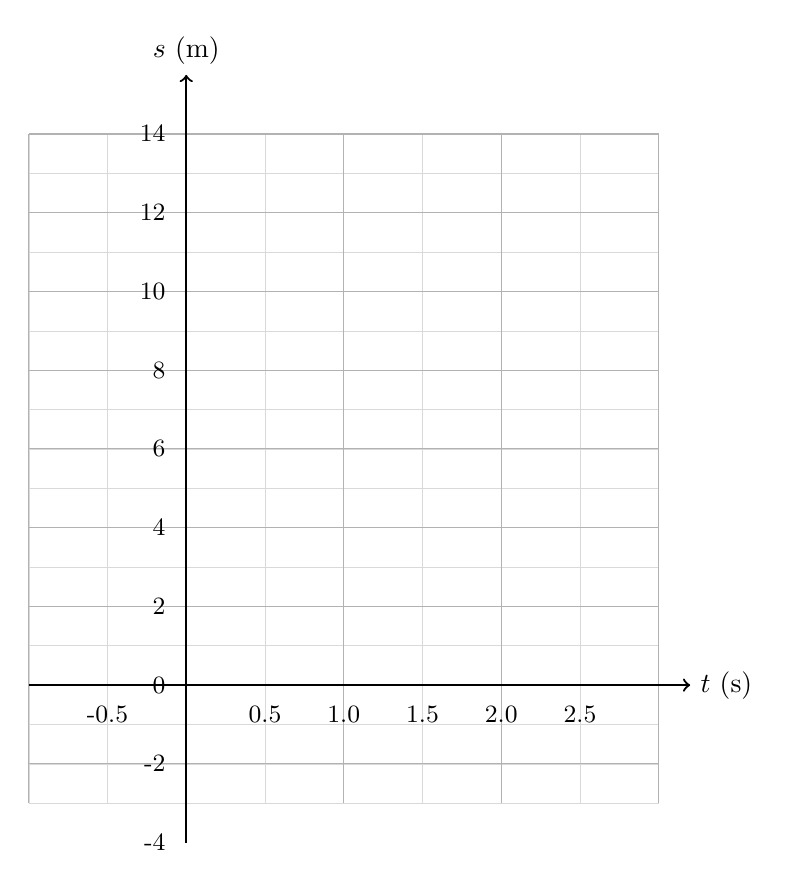
\begin{tikzpicture}[xscale=2, yscale=0.5]
  % Light grid: every 0.5 s horizontally, every 1 m vertically
  \draw[gray!30, very thin, xstep=0.5, ystep=1] (-1,-3) grid (3,14);
  % Heavy grid: every 1.0 s horizontally, every 2 m vertically
  \draw[gray!60, thin, xstep=1, ystep=2] (-1,-3) grid (3,14);
  \draw[->, thick] (-1,0) -- (3.2,0) node[right]{$t$ (s)};
  \draw[->, thick] (0,-4) -- (0,15.5) node[above]{$s$ (m)};
  % Time axis labels
  \foreach \t in {-0.5,0.5,1.0,1.5,2.0,2.5} {
    \node[below] at (\t, -0.3) {\small \t};
  }
  % Position axis labels
  \foreach \s in {-4,-2,0,2,4,6,8,10,12,14} {
    \node[left] at (-0.07, \s) {\small \s};
  }
  % Solution curve — uncomment to see the answer
  %\draw[thick, smooth, domain=-0.5:2.5, samples=80]
    %plot (\x, {-4.9*\x*\x + 12*\x + 5});
\end{tikzpicture}
\end{center}

\newpage
\item A quadratic curve fit to the data gives the equation $s = At^2 + Bt + C$ with the parameters:
$$A = -4.9, \quad B = 12, \quad C = 5$$

Comparing to the kinematic equation $s = \tfrac{1}{2}at^2 + v_0 t + s_0$, answer the following.

  \begin{enumerate}[itemsep=1.0cm]
    \item What is the initial position $s_0$?
    \item What is the initial velocity $v_0$?
    \item Calculate the acceleration $a$. (Hint: $A = \frac{1}{2}a$)
  \end{enumerate}
  \vspace{1.5cm}

\item Find the velocity at $t = 0$ numerically. Use the \textbf{average rate of change} (slope) between the points at $t = -0.5$ s and $t = 0.5$ s.
$$v(0) \approx \frac{s(0.5) - s(-0.5)}{0.5 - (-0.5)} = $$
  \vspace{2.cm}

\item Find the velocity at $t = 2.0$ s numerically. Use the average rate of change between $t = 1.5$ s and $t = 2.5$ s.
%$$v(2) \approx \frac{s(2.5) - s(1.5)}{2.5 - 1.5} = $$
  \vspace{1.5cm}

\item Using your velocity values from problems 10 and 11, calculate the average acceleration over the interval from $t = 0$ to $t = 2.0$ s.
$$a_\text{avg} = \frac{v(2) - v(0)}{2.0 - 0} = $$
  \vspace{1cm}

\item How does this value compare to the acceleration you found in problem 9(c)?

\end{enumerate}
\end{document}
